\documentclass{standalone}
\usepackage{mathrsfs}
\usepackage[x11names]{xcolor}
\usepackage{tikz, tkz-euclide}
\usepackage[american]{circuitikz}
\usepackage{siunitx}
\usepackage{textcomp}
\usetikzlibrary{arrows}
\begin{document}

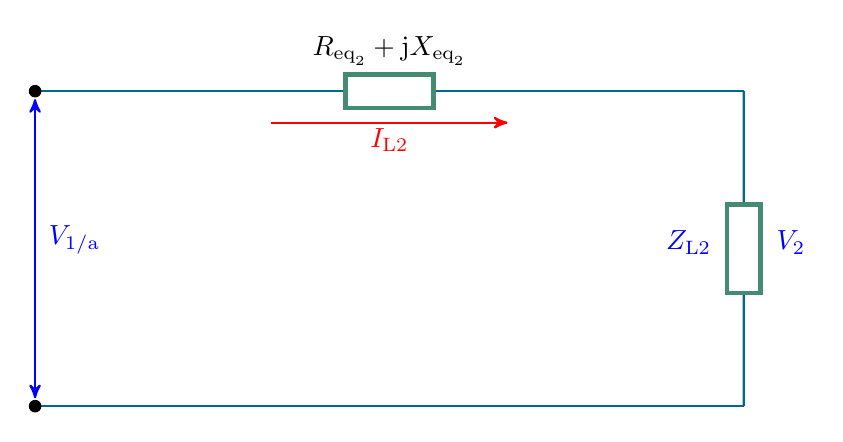
\begin{tikzpicture}[draw=DeepSkyBlue4,thick]
\draw (0,0) to (9,0);
\draw (0,4) to[european resistor, color=Aquamarine4] (9,4);
\draw (9,0) to[european resistor, color=Aquamarine4] (9,4);
\draw[draw opacity=0, fill=black] (0,0) circle (0.08);
\draw[draw opacity=0, fill=black] (0,4) circle (0.08);

\draw [<->,>=stealth',thick,blue] (0,0.1) -- (0,3.9);

\draw [->,>=stealth',thick,red] (3,3.6) -- (6,3.6);

\tkzLabelPoint[above,red](4.5,3.1){{\(I_{\mathrm{L2}}\)}}

\tkzLabelPoint[above,blue](0.5,1.8){{\(V_{\mathrm{1/a}}\)}}
\tkzLabelPoint[above,blue](8.3,1.8){{\(Z_{\mathrm{L2}}\)}}
\tkzLabelPoint[above,blue](9.6,1.8){{\(V_{2}\)}}

\tkzLabelPoint[above](4.5,4.2){{\(R_{\mathrm{eq}_{2}}+\mathrm{j}X_{\mathrm{eq}_{2}}\)}}
\end{tikzpicture}
\end{document}
